% UTF-8 encoding
% Compile with latex+dvipdfmx, pdflatex, xelatex or lualatex

\documentclass[hyperref, UTF8]{ctexart}
\usepackage{graphicx}
\usepackage{amssymb}
\usepackage{amsmath}
\usepackage{subfigure}
\usepackage{geometry}
\usepackage{caption}
\newcommand{\volt}{{\rm V}}
\newcommand{\source}{{\rm S}}
\newcommand{\ampere}{{\rm A}}
\newcommand{\ohm}{\Omega}
\newcommand{\kiloohm}{{\rm k}\Omega}
\newcommand{\watt}{{\rm W}}
\newcommand{\kilowatt}{{\rm kW}}
\title{电子学基础——第二次作业}
\author{LXQ}
\date{2019.09.24}

\geometry{left=2.0cm, right=2.0cm, top=2.5cm, bottom=2.5cm}
\linespread{1}
\begin{document}

\maketitle

\paragraph{3-2}\label{3-2}
在题图3-2所示电路中,各支路电流参考方向如图中所示。试列写求解各支路电流所需的方程组。
\begin{figure}[!htb]
\centering
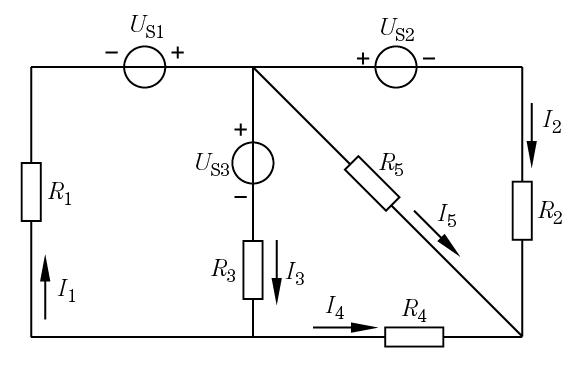
\includegraphics[width=0.388\textwidth]{p3-2.png}
\caption*{题图 3-2}
\end{figure}

\paragraph{解}
\begin{gather*}
    \left\{ \begin{aligned}
    R_1I_1-U_{\source 1}+U_{\source 3}+I_3R_3 & = 0 \\
    R_3I_3+R_4I_4-R_5I_5+U_{\source 3} & = 0 \\
    I_5R_5-I_2R_3+U_{\source 2} & = 0 \\
    I_1-I_3-I_5-I_2 & = 0 \\
    I_1+I_4-I_3 & = 0 \\
    I_5+I_4+I_2 & = 0
    \end{aligned}
    \right.
\end{gather*}

\paragraph{3-5}\label{3-5}
试列写题图3-5所示电路的回路电流方程。

\begin{figure}[!htb]
\centering
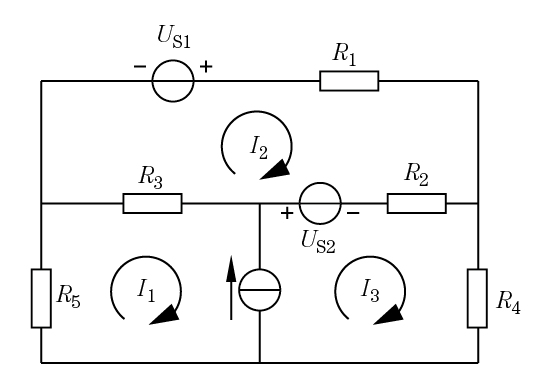
\includegraphics[width=0.361\textwidth]{p3-5.png}
\caption*{题图 3-5}
\end{figure}

\paragraph{解}
如图所示设定三个回路电流。\\
$I_2$网眼:
$$-U_{\source 1}+I_2+R_1+(I_2-I_3)R_2-U_{\source 2}+(I_2-I_1)R_3=0$$
$I_1, I_3$合网眼:
$$R_3I_1+R_3(I_1-I_2)+U_{\source 2}+R_2(I_3-I_2)+R_4I_3=0$$
电流源:
$$I_{\source 1}=I_3-I_1$$

\paragraph{3-9}\label{3-9}
用回路电流法求题图3-9所示电路中的电压$U$。
\begin{figure}[!htb]
\centering
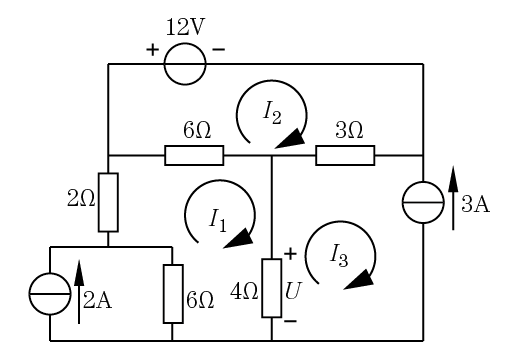
\includegraphics[width=0.337\textwidth]{p3-9.png}
\caption*{题图 3-9}
\end{figure}

\paragraph{解}如图设定三个回路电流。
\begin{gather*}
    \left\{ \begin{aligned}
    12+3(I_2-I_3)+6(I_2-I_1) &=0 \\
    6(I_1-I_2)+4(I_1-I_3)+6(I_1-2)+2I_1 &= 0 \\
    I_3 &= -3
    \end{aligned} \right.
\end{gather*}
解得
$$I_1=-1\ampere, I_2=-3\ampere, I_3=-3\ampere$$ $$\therefore U=(I_3-I_1)\cdot 2=8\volt$$

\paragraph{3-13}\label{3-13}
列写题图3-13所示电路的回路电流方程。
\begin{figure}[!htb]
\centering
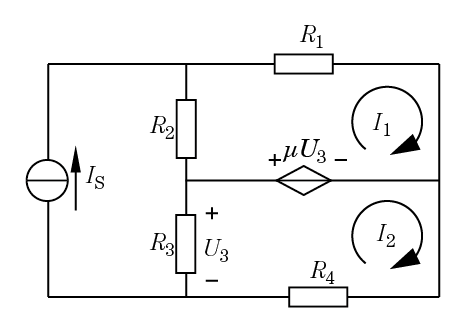
\includegraphics[width=0.312\textwidth]{p3-13.png}
\caption*{题图 3-13}
\end{figure}

\paragraph{解}如图设定两个回路电流。
\begin{gather*}
    \left\{ \begin{aligned}
    I_1R_1-\mu U_3+(I_1-I_\source)R_2 & = 0 \\
    I_2R_4-U_3+\mu U_3 &= 0 \\
    U_3 &= (I_2-I_\source)R_3
    \end{aligned} \right.
\end{gather*}

\paragraph{3-19}\label{3-19}
用节点电压法求题图3-19所示电路各支路电流。

\begin{figure}[!htb]
\centering
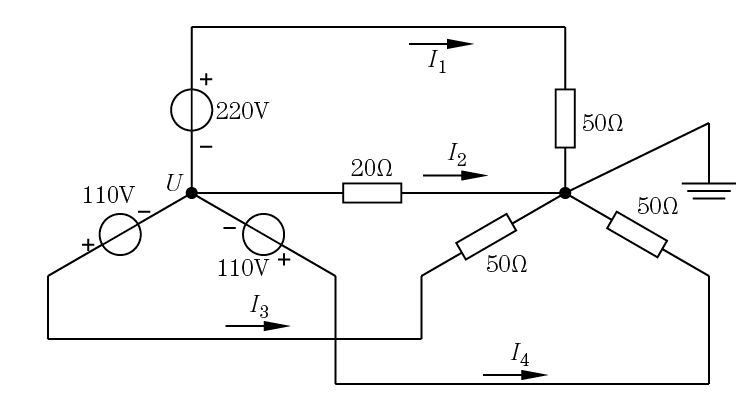
\includegraphics[width=0.503\textwidth]{p3-19.png}
\caption*{题图 3-19}
\end{figure}

\paragraph{解}
如图,将右边节点接地,左边节点电压设为$U$。则
$$\frac{U+220}{50}+\frac{U+110}{50}+\frac{U+110}{50}+\frac{U}{20}=0$$
$$\therefore U=-80\volt$$
$$\therefore I_1=2.8\ampere, I_2=-4\ampere, I_3=0.6\ampere, I_4=0.6\ampere$$

\paragraph{3-20}试用节点法求题图3-20所示电路中的电流$I$和电流源两端电压$U$。

\begin{figure}[!htb]
\centering
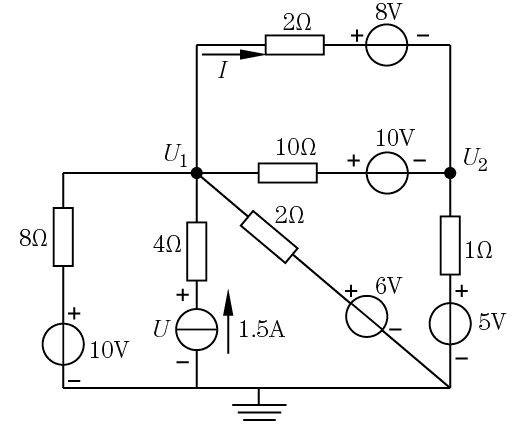
\includegraphics[width=0.344\textwidth]{p3-20.png}
\caption*{题图 3-20}
\end{figure}

\paragraph{解}
如图,将下方节点接地,另两个节点电压分别设为$U_1, U_2$,则有
\begin{gather*}
    \left\{ \begin{aligned}
    \frac{U_1-10}{8}-1.5 + \frac{U_1-6}{2} + \frac{U_1-10-U_2}{10} + \frac{U_1-8-U_2}{2} & = 0 \\
    \frac{U_2+10-U_1}{10} + \frac{U_2+8-U_1}{2} + \frac{U_2-5}{1} & = 0
    \end{aligned} \right. \\
    \therefore U_1=\frac{43}{4}\volt=10.75\volt, U_2=4.03\volt \\
    I = \frac{U_1-U_2-8}{2}=-0.64\ampere \\
    U = U_1+4 \times 1.5 = 16.75\volt
\end{gather*}

\paragraph{3-29}\label{3-29}
已知题图3-29所示电路中,$R_1=R_3=2\ohm$, $R_2=R_4=1\ohm$, $U_{\source 1}=3\volt$, $I_{\source 2}=1\ampere$。分别用回路电流法、节点电压法求解各支路电流。

\begin{figure}[!htb]
\centering
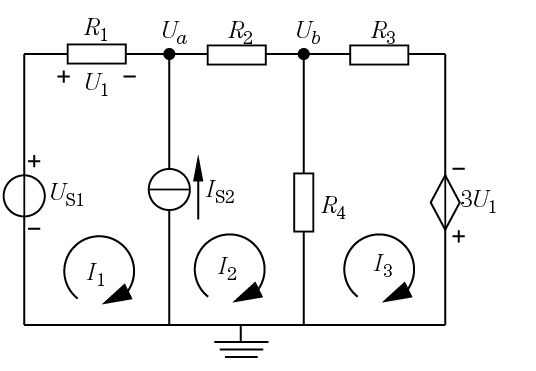
\includegraphics[width=0.357\textwidth]{p3-29.png}
\caption*{题图 3-29}
\end{figure}

\subparagraph{回路电流法}如图,设三个回路电流。
\begin{gather*}
    \left\{ \begin{aligned}
    -U_{\source 1}+R_1I_1+R_2I_2+(I_2-I_3)R_4 &= 0 \\
    (I_3-I_2)R_4+R_3I_3-3U_1 &= 0 \\
    U_1 &= R_1I_1 \\
    I_2 - I_1 &= I_{\source 2}
    \end{aligned} \right. \\
    \therefore I_1=0.8\ampere, I_2=1.8\ampere, I_3=2.2\ampere\\
     U_1=1.6\volt, I_4=I_2-I_3=-0.4\ampere
\end{gather*}
\subparagraph{节点电压法}如图,下方节点接地,上方设两个节点电压。
\begin{gather*}
    \left\{ \begin{aligned}
    \frac{U_a-U_{\source 1}}{R_1} - I_{\source 2} + \frac{U_a-U_b}{R_2} &= 0 \\
    \frac{U_b-U_a}{R_2} + \frac{U_b}{R_4} + \frac{U_b+3U_1}{R_3} & = 0 \\
    -U_a+U_{\source 1} &= U_1
    \end{aligned} \right. \\
    \therefore U_1=1.6\volt, U_a=1.4\volt, U_b=-0.4\volt \\
    \therefore I_1=0.8\ampere, I_2=1.8\ampere, I_3=2.2\ampere, I_4=-0.4\ampere
\end{gather*}

\paragraph{3-36}\label{3-36}
\subparagraph{(1)}
已知某电路的回路方程式为
\begin{gather*}
    \left\{ \begin{aligned}
    (R_1+R_2)I_1-R_2I_2 &= U_\source \\
    -R_2I_1+(R_2+R_3+R_4)I_2-R_4I_3 &= 0 \\
    -R_4I_2+(R_4+R_5)I_3 &= 0
    \end{aligned} \right.
\end{gather*}
试绘出该电路图。
\subparagraph{(2)}已知一组节点电压方程为
\begin{gather*}
    \left\{ \begin{aligned}
    5U_1-4U_2 &= -3 \\
    -4U_1+17U_2-8U_4 &= 3+I_6 \\
    17U_3-10U_4 &= 3 - I_6 \\
    -8U_2-10U_3+27U_4 &= -12 \\
    U_2-U_3 &= 6
    \end{aligned} \right.
\end{gather*}
试绘出相应的电路图。

\paragraph{解}
\subparagraph{(1)}如图3-36 (1)所示。

\begin{figure}[!htb]
\centering
\begin{minipage}[t]{0.309\textwidth}
\centering
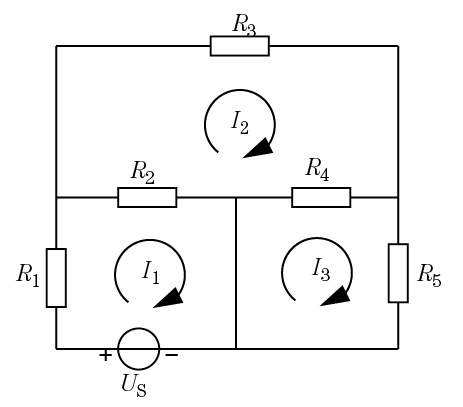
\includegraphics[width=1\textwidth]{p3-36-1-sol.png}
\caption*{(1)}
\end{minipage}
\begin{minipage}[t]{0.505\textwidth}
\centering
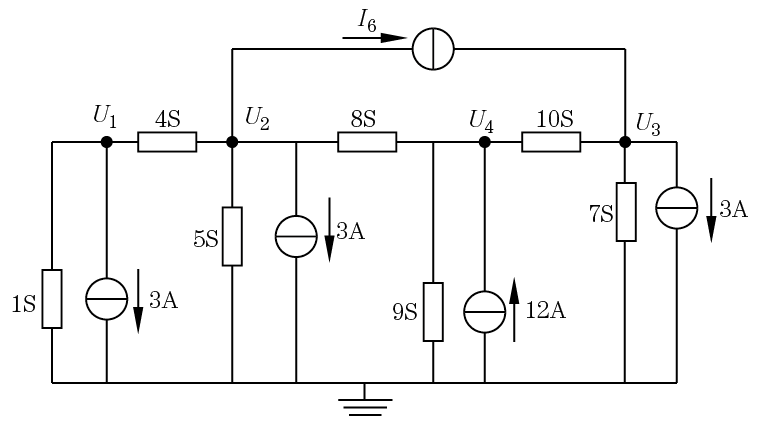
\includegraphics[width=1\textwidth]{p3-36-2-sol.png}
\caption*{(2)}
\end{minipage}
\caption*{图 3-36}
\end{figure}

\subparagraph{(2)}将方程组改写为矩阵形式
\begin{gather*}
    \left[ \begin{matrix}
    5 & -4 & 0 & 0 \\ -4 & 17 & 0 & -8 \\ 0 & 0 & 17 & -10 \\ 0 & -8 & -10 & 27
    \end{matrix} \right]
    \left[ \begin{matrix}
    U_1 \\ U_2 \\ U_3 \\ U_4
    \end{matrix} \right]
    =
    \left[ \begin{matrix}
    3 \\ 3+I_6 \\ 3-I_6 \\ -12
    \end{matrix} \right] \\
    \therefore
    \left[ \begin{matrix}
    4+1 & -4 & 0 & 0 \\ -4 & 4+8+5 & 0 & -8 \\ 0 & 0 & 10+7 & -10 \\ 0 & -8 & -10 & 8+10+9
    \end{matrix} \right]
    \left[ \begin{matrix}
    U_1 \\ U_2 \\ U_3 \\ U_4
    \end{matrix} \right]
    =
    \left[ \begin{matrix}
    3 \\ 3+I_6 \\ 3-I_6 \\ -12
    \end{matrix} \right] \\
\end{gather*}
则可得电路图如图3-36 (2)所示。

\paragraph{4-2}\label{4-2}
题图4-2所示电路中,已知某一瞬间流过电感的电流为$I_L$。求此时流过电阻$R_2$的电流$I$。

\begin{figure}[!htb]
\centering
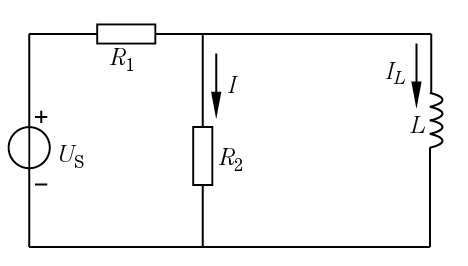
\includegraphics[width=0.312\textwidth]{p4-2.png}
\caption*{题图 4-2}
\end{figure}

\paragraph{解}
\begin{gather*}
U_\source = (I+I_L)R_1+IR_2 \\
\therefore I=\frac{U_\source-I_LR_1}{R_1+R_2}
\end{gather*}

\paragraph{4-3}\label{4-3}
用叠加定理求题图4-3所示电路的电压$U_o$。

\begin{figure}[!htb]
\centering
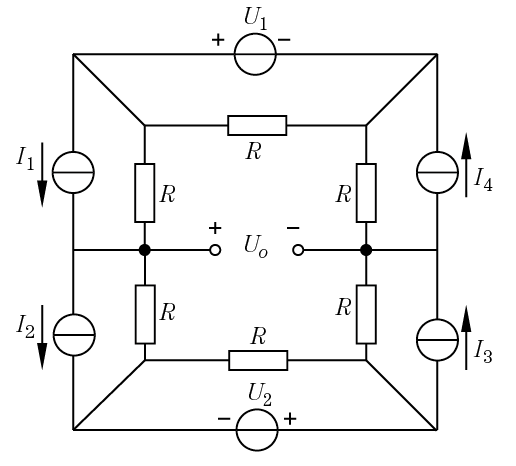
\includegraphics[width=0.344\textwidth]{p4-3.png}
\caption*{题图 4-3}
\end{figure}

\begin{figure}[!htb]
\centering
\begin{minipage}[t]{0.343\textwidth}
\centering
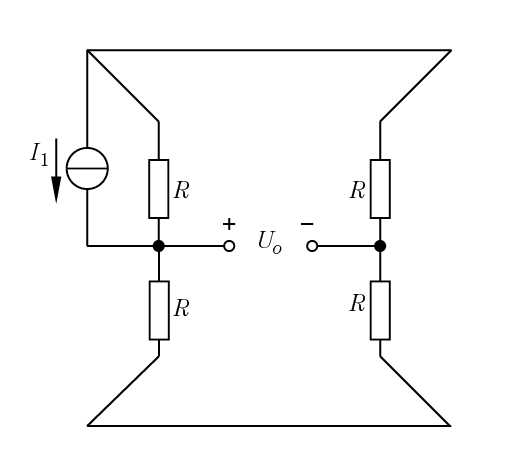
\includegraphics[width=1\textwidth]{p4-3-sol1.png}
\caption*{(1)}
\end{minipage}
\begin{minipage}[t]{0.337\textwidth}
\centering
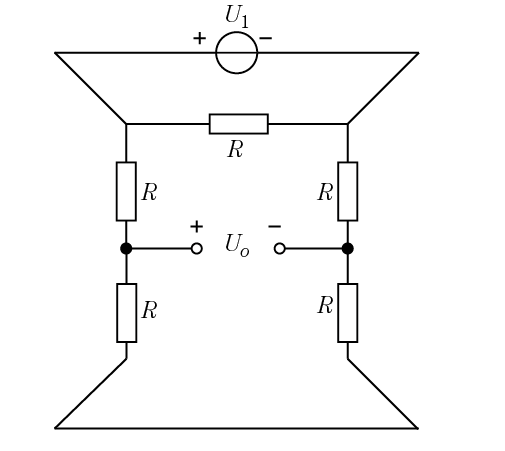
\includegraphics[width=1\textwidth]{p4-3-sol2.png}
\caption*{(2)}
\end{minipage}
\caption*{图 4-3}
\end{figure}

\paragraph{解}
仅$I_1$作用时,电路图如图4-3 (1)所示,此时$R$与$3R$并联。则
$$U_{oI_1}=\frac{1}{2}RI_1$$
仅$I_2, I_3, I_4$作用时,同理,有
$$U_{oI_2}=-\frac{1}{2}RI_2, U_{oI_3}=-\frac{1}{2}RI_3,
U_{oI_4}=\frac{1}{2}RI_4$$
仅$U_1$作用时,如图4-3 (2)所示,此时$R$与$4R$并联。则
$$U_{oU_1}=\frac{U\cdot 2R}{4R}=\frac{1}{2}U_1$$
仅$U_2$作用时同理,
$$U_{oU_2}=-\frac{1}{2}U_2$$
则共同作用时
$$U_o=\frac{1}{2}(U_1-U_2)+\frac{R}{2}(I_1-I_2-I_3+I_4)$$

\paragraph{4-9}\label{4-9}
题图4-9所示电路中,已知$i_{\source 1}=i_{\source 2}=5\ampere$, $i=0$;当$i_{\source 1}=8\ampere$, $i_{\source 2}=6\ampere$时,$i=4\ampere$。求当$i_{\source 1}=3\ampere$, $i_{\source 2}=4\ampere$时电流$i$的值。

\begin{figure}[!htb]
\centering
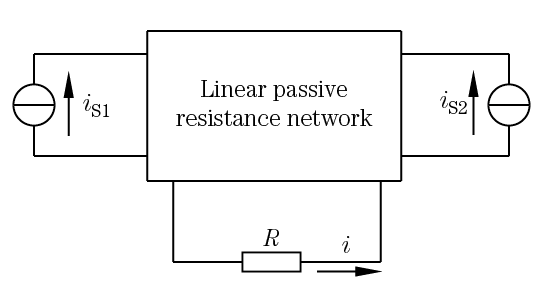
\includegraphics[width=0.370\textwidth]{p4-9.png}
\caption*{题图 4-9}
\end{figure}

\paragraph{解}
由叠加定理,$i$是$i_{\source 1}$, $i_{\source 2}$的线性组合。则可设$i=\lambda i_{\source 1} + \mu i_{\source 2}$。由题中数据:
\begin{gather*}
    \left\{ \begin{aligned}
    0 &= 5 \lambda + 5 \mu \\
    4 &= 8 \lambda + 6 \mu
    \end{aligned} \right. \\
    \therefore \lambda = 2, \mu = -2 \\
    \therefore i_{\source 1}=3\ampere, i_{\source 2}=4\ampere \text{时}, i=-2\ampere
\end{gather*}

\paragraph{4-10}\label{4-10}
题图4-10所示电路中,已知电流源$I_{\source 1}=2\ampere$, $I_{\source 2}=3\ampere$。当$3\ampere$的电流源断开时,$2\ampere$的电流源输出功率为$28\watt$,这时$U_2=8\volt$。当$2\ampere$的电流源断开时,$3\ampere$的电流源输出功率为$54\watt$,这时$U_1=12\volt$。试求两个电流源同时作用时,每个电流源输出的功率。

\begin{figure}[!htb]
\centering
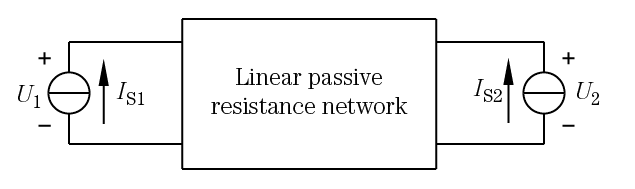
\includegraphics[width=0.423\textwidth]{p4-10.png}
\caption*{题图 4-10}
\end{figure}

\paragraph{解}
$I_{\source 2}$断开时,$P_{\rm out}=28\watt$,则此时$U_1=14\volt$。\\

$I_{\source 1}$断开时,$P_{\rm out}=54\watt$,则此时$U_2=18\volt$。\\

$\therefore$共同作用时
$$ U_1=14+12=26\volt $$
$$ U_2=18+8=26\volt $$
$$ P_{\rm out1}=U_1I_1=52\watt $$
$$ P_{\rm out2}=U_2I_2=78\watt $$

\end{document} 